\documentclass[french]{article}

	\usepackage[in]{fullpage}
	\usepackage[utf8]{inputenc}
	\usepackage[T1]{fontenc}
	\usepackage{lmodern}
	\usepackage[main=french]{babel}

	\usepackage{graphicx}
	\usepackage{amsmath,amsfonts}
	\usepackage{mathrsfs}
	\usepackage{stmaryrd}
	\usepackage[top=1in, bottom=1.25in, left=1.25in, right=1.25in]{geometry}

	\title{Construction et modélisation d'un réseau routier}
	\author{Louis-Brahim BEAUFORT}

	\newtheorem{thm}{Théorème}
	\newtheorem{déf}{Définition}
	\newtheorem{prop}{Propriété}
	\newtheorem{rem}{Remarque}

\begin{document}

  \maketitle

  L'objectif de ce travail est de présenter une modélisation fidèle de l'établissement d'un réseau routier entre plusieurs villes. Plus précisément, étant données une carte d'une région ainsi que les coordonnées de points, on tentera de relier ces différents lieux par un réseau de routes. Par souci de simplicité, on ne s'intéresse pas ici à modéliser les flots de véhicules pouvant emprunter ces routes pour se concentrer uniquement sur leur tracé.

	\section{Construction du graphe initial}

		Soit $f:\mathbb{R}^{2} \longmapsto \mathbb{R}$ une fonction qui à tout point du plan associe son altitude, et $(v_{0},...,v_{n-1}) \in \mathbb{R}^{3}$ une suite de points de l'espace représentant des villes (par leurs coordonnées). On adjoint à ces villes un graphe $G = (V,R)$ où $V=\{v_{0},...,v_{n-1}\}$ est l'ensemble des villes et $R \in V \times V$ représente les routes les reliant. Le premier objectif est de construire algorithmiquement $R$. \newline
		Pour cela, on construit une représentation du terrain plus maniable que la fonction altitude à l'aide d'une grille : le terrain est représenté maintenant par un graphe fini $T$ que l'on prend de forme carrée, défini par sa résolution et sa taille, où on identifie une région du plan à un point de l'espace que l'on relie à huit autres points adjacents. Cette tâche est réalisée par l'algorithme \verb?discretisation? de complexité linéaire en la résolution. \newline

		\begin{figure}[h]
			\centering
			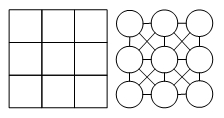
\includegraphics[width=5cm]{Pics/Disc.jpg}
			\caption{Exemple de discrétisation de résolution 3}
		\end{figure}

		On définit alors la \emph{carte de la région représentée par f contenant les villes $(v_{0},...,v_{n-1})$} comme le triplet $(f,G,T)$ représenté par la classe \verb?Map?. Les graphes sont représentés par des listes d'adjacence.
		\newline
		\newline
		On désire maintenant, à partir de $V$, construire $R$ : on utilise pour cela l'algorithme de Dijkstra. Cet algorithme permet de résoudre le problème de plus court chemin. On procède comme suit : chaque ville $v$ est associée à l'un des sommets du graphe $T$ réalisant la plus petite distance à $v$ (on l'obtient à l'aide d'un parcours avec \verb?pos?) puis on relie ces sommets entre eux en appliquant à chaque paire l'algorithme de plus court chemin; ce processus est réalisé par \verb?init?. La suite d'arêtes de $T$ reliant deux villes définit l'arête de $G$ reliant ces villes.\newline
		L'algorithme de Dijkstra \verb?dijkstra? demande pour une complexité optimale la mise en place d'une structure de file de priorité, qui est implémentée sous la forme de la classe \verb?Heap? par un tas min binaire. La procédure complète atteint une complexité en $O(n^{2}r^{2}\ln(r))$, étant réalisée sur le graphe $T$, creux. \newline
		Enfin, cet algorithme s'applique sur un graphe pondéré (par des poids positifs). La pondération d'une arête est donnée par la formule : $\omega(a) = \alpha l(a) + \beta V(a,f)$ où $\alpha, \beta$ sont des constantes, $l(a)$ désigne la longueur de l'arête (selon la distance euclidienne entre les sommets qu'elle joint) et $V(a,f)$ le volume d'un prisme de hauteur $l(a)$ et de base un triangle rectangle dont les deux côtés les plus petits ont pour longueur respectivement une largeur $l$ et la variation d'altitude $|\Delta f|$ entre les deux sommets. Le choix de cette pondération sera expliqué par la suite.

		\begin{figure}[h]
			\centering
			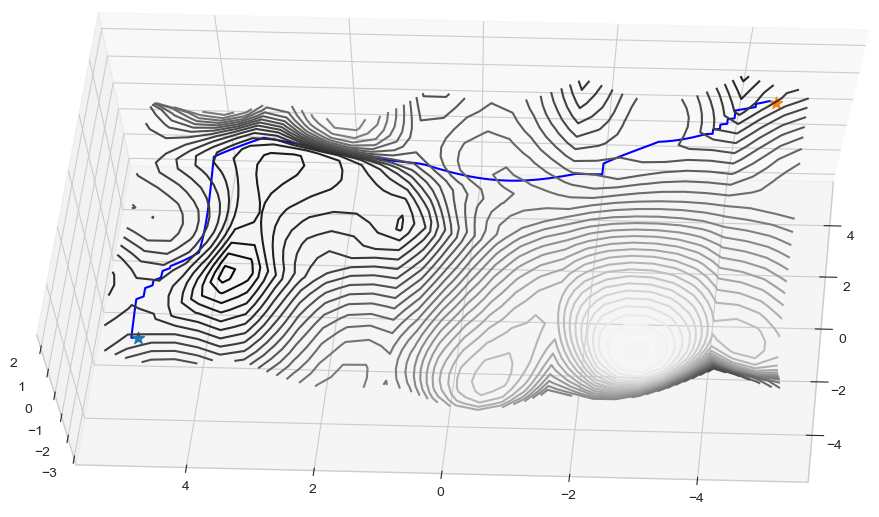
\includegraphics[width=5cm]{Pics/lacets.png}
			\caption{Un exemple d'exécution de \verb!init! pour T de taille 5000, résolution 50, $n = 2$, $\beta = 10 \alpha$, $l=6$}
		\end{figure}

		A l'issue de cette procédure, on obtient bien notre graphe $G$ complété. En revanche, il peut arriver que deux des arêtes de $G$ contiennent plusieurs arêtes communes, ce qui se concevrait comme plusieurs routes superposées. Cette superposition conduit à une erreur lors du calcul d'une pondération de $G$ obtenue à partir d'une pondération de $T$ : certaines arêtes de $T$ sont comptées plusieurs fois. Pour remédier à ce problème, on introduit la procédure \verb?cree_jonctions?.\newline
		Le principe est de considérer chaque arête de $G$ comme une suite de sommets de $T$ et de trouver tous les points d'intersection entre deux arêtes de $G$. Chacun de ces points est ensuite susceptible d'être ajouté à $G$ sous le statut de \emph{jonction}. Les deux arêtes considérées sont ensuite scindées en quatre arêtes. La complexité de cet algorithme assez brutal est un $O(r^{2}n^{5})$ dans le pire cas mais en pratique difficile à évaluer (on ne sait pas si les arêtes ont tendance à être superposées ou non).

		\begin{figure}[h]
			\centering
			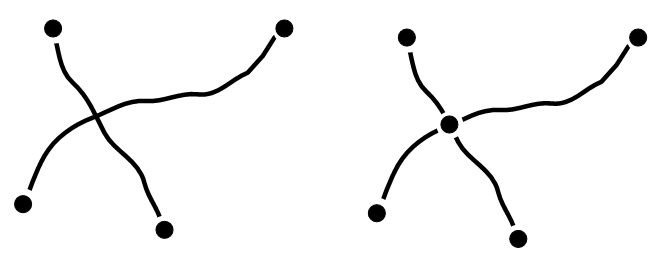
\includegraphics[width=5cm]{Pics/jonct.jpg}
			\caption{Avant/Après \verb?cree_jonctions?}
		\end{figure}

		Cette opération est susceptible de faire apparaître des boucles, des arêtes doublons dans le graphe qui sont éliminées par \verb?supprime_nuls? et \verb?supprime_doubles?. A son issue, on fait également disparaître les jonctions dont le degré vaut exactement 2 (il n'y a pas lieu de jonction alors) avec \verb?fusion? ou 1 (des impasses) avec \verb?tailladeur?.


		\section{Coûts}

		Maintenant que nous avons un réseau digne de ce nom, nous allons pouvoir tenter d'en extraire un réseau optimal. Oui, mais que veut dire optimal ?\newline
		\newline
		On définit le coût de construction d'une arête de $T$ comme étant sa pondération $\omega = \alpha l(a) + \beta V(a,f)$ déjà définie dans la partie précédente. La contribution de $l(a)$ est le coût de pose de la route, et la contribution de $V(a,f)$ s'interprète comme étant le volume de roche à creuser dans la montagne pour rendre la pose d'une route droite possible. En particulier, cette dernière contribution explique pourquoi la route obtenue évitait les variations d'altitude et décrivait des lacets. On élargit ensuite cette définition à une arête de $G$ puis à $G$ tout entier en passant à la somme.\newline
		\newline
		A ce coût de construction on va opposer un coût d'utilisation décrivant le point de vue d'un utilisateur de la route. On commence par fixer une vitesse de circulation$v_{max}$ et on définit pour une arête $a$ de $T$ la vitesse de circulation sur $a$ $v(a) = v_{max} $ si la pente de cette arête est assez faible et $v(a) = 0$ sinon. Une route trop pentue est interdite d'accès. On en déduit pour toute arête de $T$ le temps de parcours de cette arête, puis le temps de parcours d'une arête de $G$.\newline
		A ce temps on ajoute un temps additionnel dû aux virages rencontrés : celui-ci représente la différence entre le temps de parcours obtenu en roulant à $v_{max}$ et celui obtenu en décélérant, passant le virage, puis accélérant. La vitesse maximale de traversée du virage s'obtient à partir de son rayon de courbure $R$ et du coefficient de frottement de la route $f$ par $v < \sqrt{Rgf}$. \newline
		On souhaite ensuite calculer pour une arête de $T$ l'énergie dépensée pour la traverser. La formule obtenue est (on rappelle que v est ici fixée !) : \newline
		$\Delta E = \Delta E_{c} + \Delta E_{p,pes} + E_{roulement} + E_{frott} = m g (1+c_{r}) \Delta z + S \rho v^{3} \Delta t$ \newline
		Avec $c_{r}$ le coefficient de frottement de roulement, $g$ la pesanteur, $m$  la masse du véhicule, $\rho$ la masse volumique de l'air et $S$ la surface projetée du véhicule. On considère également que si cette expression a une évaluation négative, on prend l'énergie nulle (le véhicule ne possède pas de dynamo).\newline
		On définit alors le coût d'usage d'une arête de $T$ comme le produit de cette énergie et du temps de parcours. On l'étend ensuite à $G$ tout entier de la manière suivante : le coût d'usage de $G$ est défini comme la somme double pour deux sommets de $G$ du coût d'usage du plus court chemin reliant ces arêtes. Il correspond au coût d'utilisation car représente les plus courts chemins qui vont être utilisés.\newline
		Le graphe muni de ce coût d'usage se comporte de façon complexe : il ne s'agit pas d'une simple pondération ! Une propriété élémentaire d'un tel coût est par exemple que le graphe complet sera toujours optimal pour ce coût et plus généralement enlever des arêtes augmente le coût. Il est donc hors de question d'utiliser un algorithme de recherche d'arbre de poids minimal pour tenter de trouver un optimum. De façon générale, une recherche bibliographique montre que peu se sont intéressés au sujet... \newline
		Le calcul de ce coût est également difficile : il demande de trouver la liste des plus courts chemins entre chaque sommet. Ce calcul fut fait à partir de l'algorithme de Floyd-Warshall mais se fait maintenant à partir de \verb?dijkstra_generalise? pour une efficacité accrue. Le temps de calcul est un $O(n^{2}\log(n))$. Aussi, pour éviter d'avoir à le calculer plusieurs fois, on associe à $G$ son coût d'usage de manière permanente. Cela suggère de devoir le mettre à jour à chaque modification de $G$. Cependant, une modification de $G$ implique une mesure de la variation de son coût, donc le calcul devra de toute façon être fait. Il est réalisé par la méthode \verb?update_fl?.
		\newline
		L'objectif est alors de concilier les deux coûts ainsi définis. Le consensus adopté par la suite sera une moyenne géométrique.
		\section{Réduction}

		Nous avons donc un graphe à réduire sans vraiment de méthode miracle.

			\subsection{Élimination des arêtes inutiles}

				La première optimisation à laquelle on pourrait penser est une suppression des arêtes ne faisant partie d'aucun plus court chemin. On montre qu'une telle suppression laisse le coût d'usage invariant mais fait diminuer le coût de construction : une telle réduction est donc envisageable. \newline
				On utilise alors une astuce pour éviter de devoir recalculer la liste des plus courts chemins : lors du calcul du coût d'usage, on attribue à chaque route le nombre de plus courts chemins auxquels elle appartient (attribut \verb?Road.flux?). On supprime alors toutes les routes pour lesquelles ce nombre est nul. Cette méthode a une complexité en $O(n^{2})$. \newline
				On pourrait penser au premier abord que ces routes n'existent pas : après tout, elles faisaient partie d'un plus court chemin lorsqu'on les a construites au début. Mais depuis la définition du coût a changé, et on se rend compte que en général de nombreuses routes en font partie.

			\subsection{Élimination des $K_{3}$}

				Une autre solution possible consiste à chercher les sous-graphes triangulaires de $G$. Si l'une des arêtes est assez longue devant les deux autres, on l'enlève. Pour un tel sous-graphe constitué des arêtes $a,b,c$, où $a_{c}$ et $a_{u}$ désignent respectivement les coûts de construction et d'usage de $a$, on fait varier $x \in [0,1]$ et on cherche quand  $(1+x) c_{c} c_{u} > (a_{c} + b_{c})(a_{u} + b_{u})$. Si c'est le cas, on retire c. On cherche ensuite le minimum du compromis en fonction de $x$. Complexité : $O(n^{6})$ dans le pire cas, atteint lorsque le nombre de sous-graphe triangulaires vaut $\binom{n}{3}$ (par exemple pour le graphe complet).
			\subsection{Solution optimale par backtracking}

				Il est également possible de chercher directement la vraie solution au lieu de se lancer dans des algorithmes hasardeux. En considérant l'ensemble $R$ des arêtes de $G$, on conçoit \verb?sol_opt? un algorithme fournissant la solution optimale par backtracking. Le principe est le suivant : pour un certain $R$, on considère récursivement toutes les parties de $R$ contenant $|R|-1$ éléments et on choisit parmi celles ci et $R$ lui-même le graphe réalisant un minimum du compromis. Si un sous-graphe strict de $R$ est choisi, on recommence la manoeuvre récursivement, sinon on renvoie directement $R$. Notamment à cause du calcul du coût d'usage, la complexité de cet algorithme atteint des proportions gigantesques : au moins $O((|R|!)^{2})$. Dans la pratique, on ne considère souvent pas de sous-graphes auxquels on a retiré beaucoup d'arêtes pour cause de problèmes de connexité, ce qui améliore le temps d'exécution, mais cela reste trop.

			\subsection{Probabilisation selon le paradigme du recuit simulé}

				On cherche donc à améliorer l'algorithme exact précédent afin qu'il soit utilisable en un temps raisonnable. On va chercher alors à le probabiliser en utilisant la méta-heuristique du recuit simulé : lorsque l'on retire des arêtes de $G$, on le fait aléatoirement et on les stocke dans une liste, et si cette liste n'est pas vide on peut avec équiprobabilité ajouter ou retirer une arête de $G$. De plus, pour s'assurer de la convergence de l'algorithme, on n'accepte de retirer ou ajouter une arête tirée au hasard que si elle diminue le compromis ou, si ce n'est pas le cas, avec une certaine probabilité diminuant avec le temps (ie. le nombre d'itérations). Cette diminution laisse le temps à l'algorithme de s'extraire d'éventuels minima locaux, du moins en théorie. La tâche est effectuée par \verb?recuit?. La complexité par itération de l'algorithme est en $O(n^{2})$ ce qui permet de le répéter un bon nombre de fois.

	\paragraph{Conclusion}

		Comme le montrent plusieurs résultats (présentés en annexe), les algorithmes présentés permettent de trouver plusieurs solutions au problème posé. Les réseaux présentés donnent une idée de ce que pourrait être le réseau réel et sont agréables à l'oeil.\newline
		Les deux alternatives proposées, déterministe et probabiliste, fournissent en général des résultats semblables. Il semblerait toutefois que le seul algorithme vraiment efficace soit \verb?elimination?. L'application de la méthode du recuit simulé fournit des résultats satisfaisants, légèrement meilleurs (1,06\%)que ses alternatives déterministes. On constatera cependant que du fait de l'abstraction des coûts utilisés une solution plus coûteuse peut être parfois plus attrayante qu'une moins coûteuse. \newline
		Cependant, l'approximation du terrain par une grille induit pour des valeurs de la résolution trop importantes des erreurs d'appréciation des distances; une étude expérimentale indique que cette erreur est linéaire en $\frac{1}{r}$. Sa correction implique toutefois l'exécution de l'algorithme sur des valeurs de pas très faible, ce qui est irréalisable du point de vue temporel. \newline
		Une première façon d'améliorer ce modèle serait de prendre en compte la possibilité d'édification de ponts et tunnels. Cependant, ceux-ci demanderaient une modélisation du terrain en trois dimensions, ce qui serait coûteux.\newline
		Une deuxième façon serait de coupler les résultats de l'algorithme à la théorie des problèmes de flot, en faisant intervenir par exemple une largeur des routes variable.

	\appendix

		\paragraph{Bibliographie}

			\begin{itemize}

				\item CORMEN,LEISERSON,RIVEST : Introduction à l'algorithmique : Dunod, 2002, pages 577-582

				\item CORMEN,LEISERSON,RIVEST : Introduction à l'algorithmique : Dunod ,2002, pages 609-614

				\item WEISBUCH Gérard : Dynamique des systèmes complexes, Chapitre 9 : http://www.lps.ens.fr/~weisbuch/livre/b9.html

			\end{itemize}

		\paragraph{Galerie}

			Les résultats sont organisés de la façon suivante : de gauche à droite, de haut en bas,
			\begin{itemize}
				\item Le graphe complet obtenu après \verb?init?
				\item Ce dernier graphe après \verb?normalisation? ie. l'ajout de jonctions
				\item Le graphe normalisé après être passé par les trois premiers algorithmes de réduction (déterministes)
				\item Le graphe normalisé après être passé par le dernier algorithme de réduction (probabiliste)
			\end{itemize}
			Ces deux derniers sont ensuite reproduits en trois dimensions au dessous, dans l'ordre.

			\newpage

			\begin{figure}[H]
				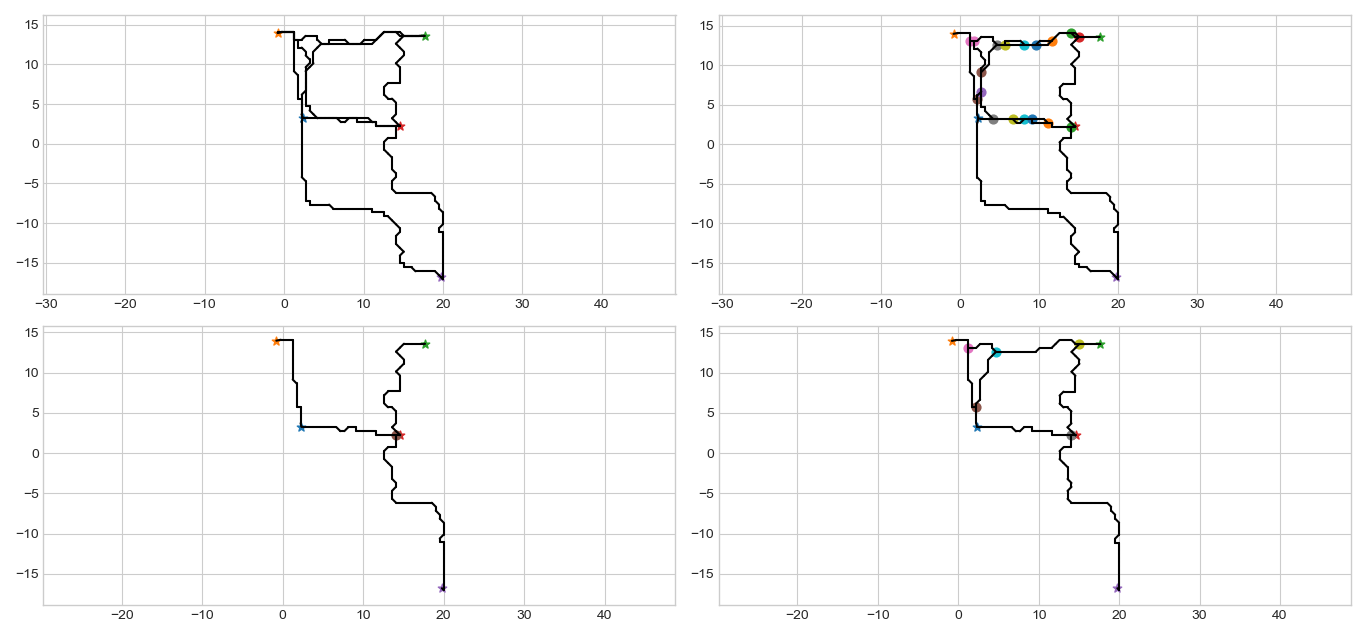
\includegraphics[width=5cm]{Pics/g11.png}
			\end{figure}

			\begin{figure}[H]
				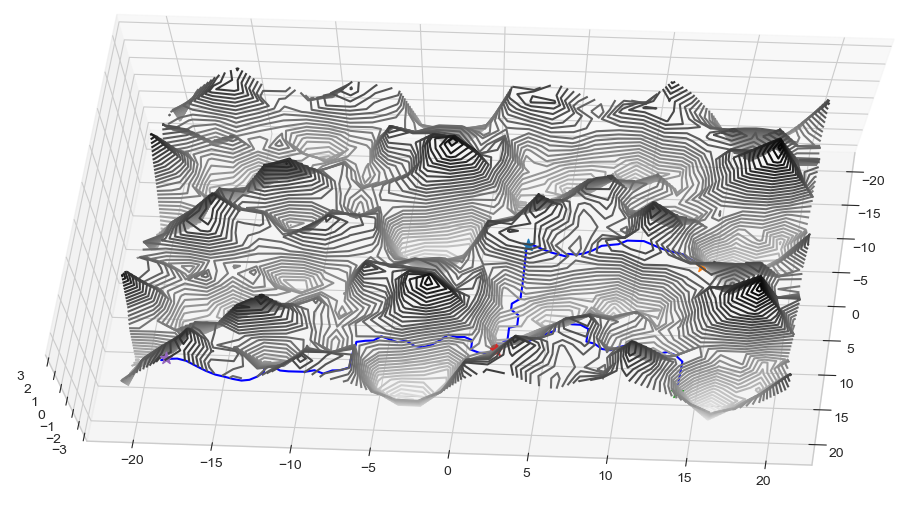
\includegraphics[width=5cm]{Pics/g12.png}
			\end{figure}

			\begin{figure}[H]
				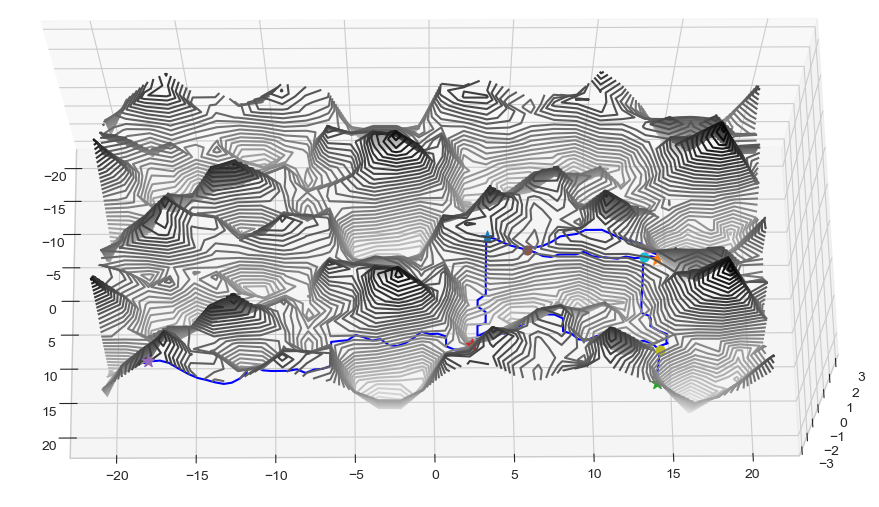
\includegraphics[width=5cm]{Pics/g13.png}
			\end{figure}

			\newpage

			\begin{figure}[H]
				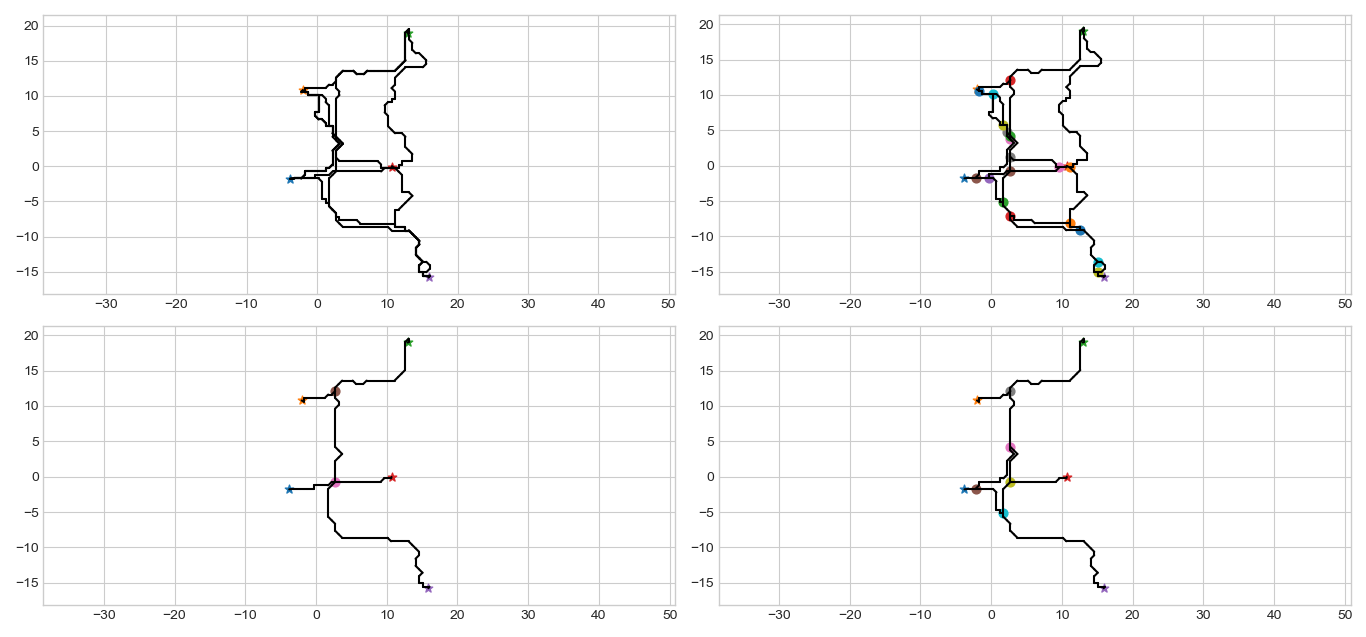
\includegraphics[width=5cm]{Pics/g21.png}
			\end{figure}

			\begin{figure}[H]
				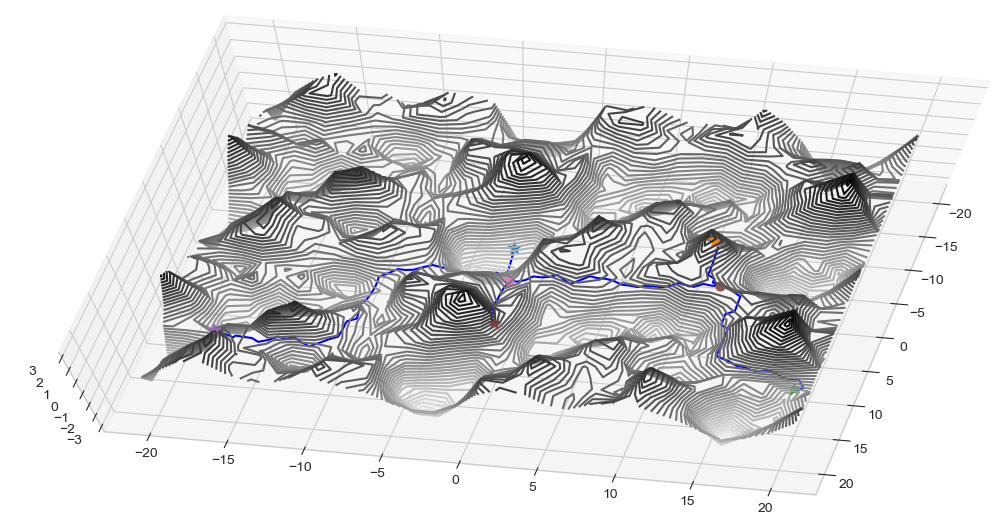
\includegraphics[width=5cm]{Pics/g22.png}
			\end{figure}

			\begin{figure}[H]
				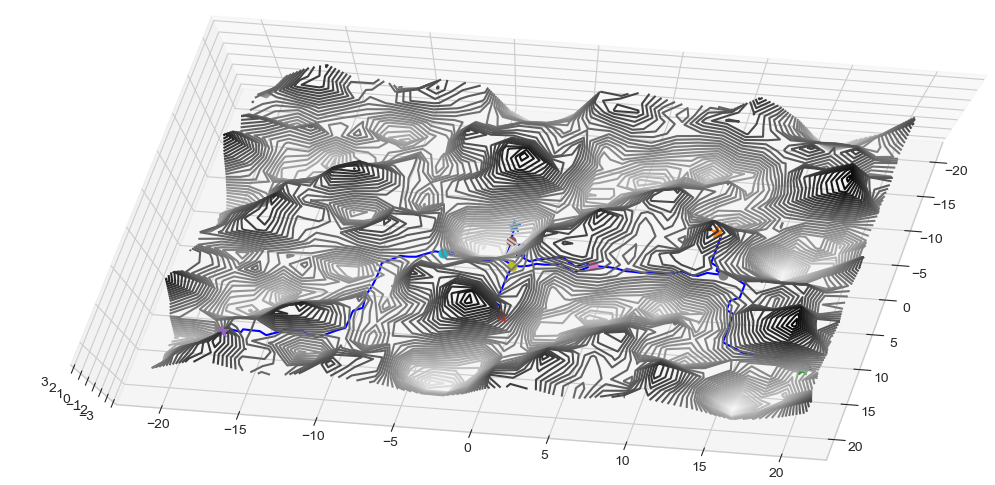
\includegraphics[width=5cm]{Pics/g23.png}
			\end{figure}

			\newpage

			\begin{figure}[H]
				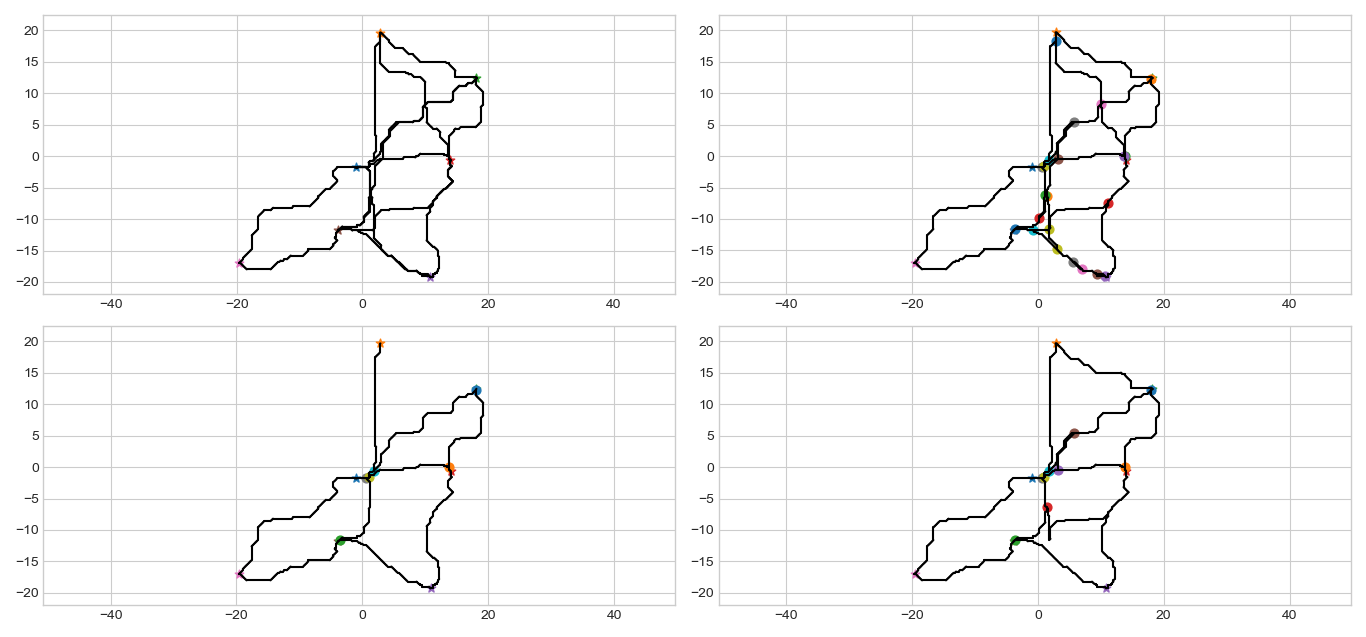
\includegraphics[width=5cm]{Pics/g31.png}
			\end{figure}

			\begin{figure}[H]
				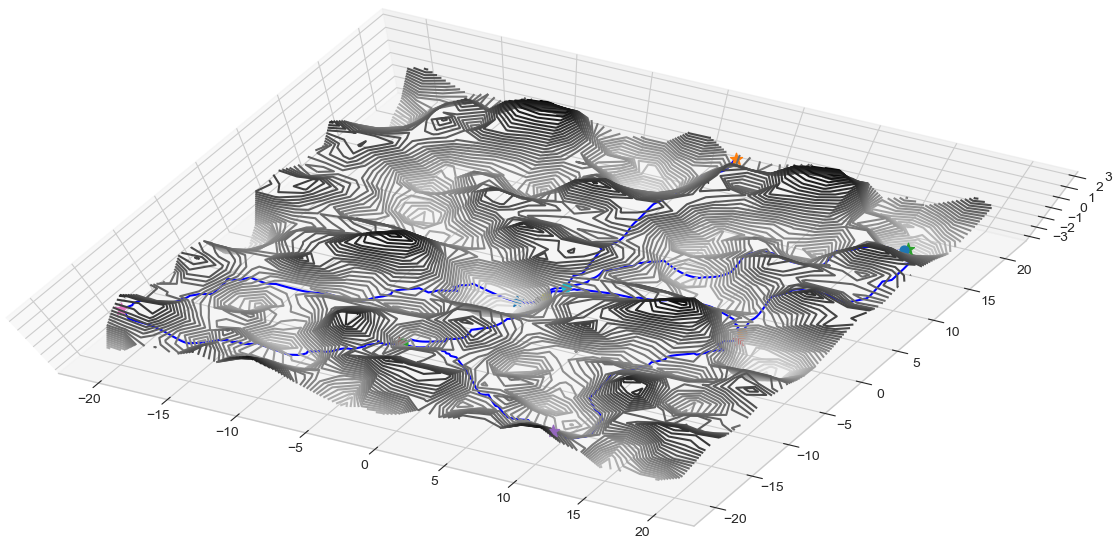
\includegraphics[width=5cm]{Pics/g32.png}
			\end{figure}

			\begin{figure}[H]
				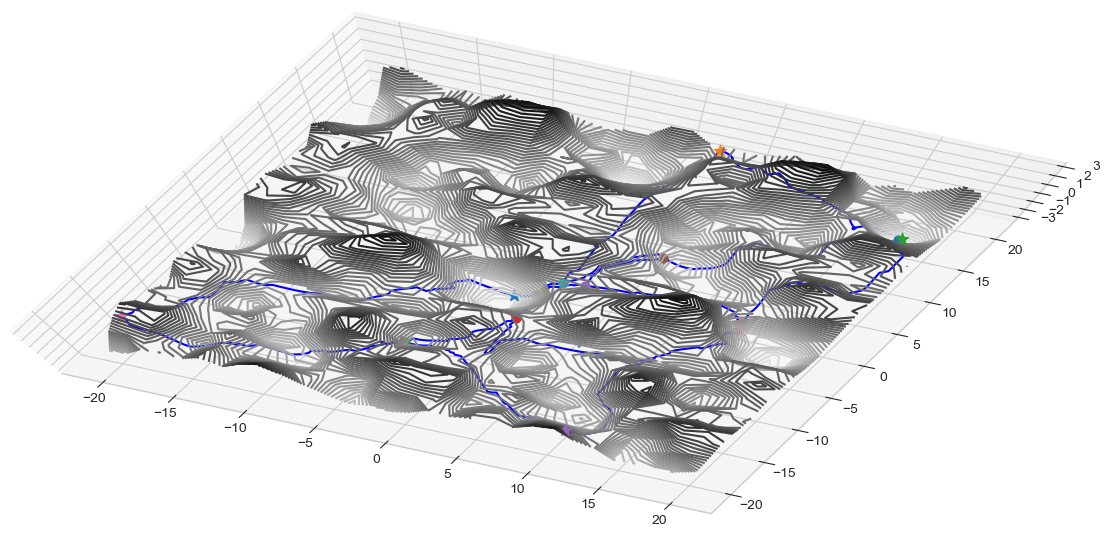
\includegraphics[width=5cm]{Pics/g33.png}
			\end{figure}

			\newpage

\end{document}
